\documentclass{deliverablereport}

\deliverable{UI}{vis3d}
\deliverydate{31/08/2018}
\duedate{31/08/2018 (M36)}
\author{Benjamin Ragan-Kelley, Vidar Tonaas Fauske, Marcin Kostur}

\begin{document}
\maketitle
\tableofcontents

%%%%%%%%%%%%%%%%%%%%%%%%%%%%%%%%%%%%%%%%%%%%%%%%%%%%%%%%%%%%%%%%%%%%%%%%

\section{Introduction}

The \href{https://jupyter.org}{Jupyter Notebook} is a web application
that enables the creation and sharing of executable documents
containing live code, equations, visualisations and explanatory text.
In particular, Jupyter is used actively for interactive and exploratory computations,
often involving visualisation of data.

Because Jupyter is a web-based application,
it can benefit from developments in the wider community development of visualisation tools for the web, in which there is a lot of activity.
The primary task for developing visualisation tools in Jupyter is providing tools for connecting
"kernel" code, where the user's code runs,
to visualisation code running in the browser.
Two-dimensional visualisation in Jupyter is an area with popular and well-established tools
such as \href{https://matplotlib.org}{matplotlib}, \href{https://bokeh.pydata.org/}{bokeh}, and \href{https://altair-viz.github.io}{altair},
but there have been fewer mature solutions for three-dimensional visualisation in Jupyter.
It is an area of active exploration,
so we first set out to identify the current state of the art for 3D visualisation in Jupyter,
and determine where our efforts could best be placed.
We did this in the form of a report on the landscape of 3D visualisation in Jupyter in 2017.

The Jupyter ecosystem includes a collection of projects called `Jupyter Widgets,'
which is a widely used system for providing bidirectional communcation
between the kernel and the browser.
The widgets provide a powerful and extensible system and we chose to use it as our basis for development of new visualisation tools,
and focused our efforts with existing tools on improving compatibility with the Jupyter Widgets system.

For this deliverable, we aim to accomplish two main tasks: To better
understand the existing landscape of community efforts for three-dimensional
visualisation in notebooks and to contribute where we may have the best
impact, whether it be in contributing to existing projects or creating new
tools. We have accomplished both. In particular, we have helped improve the
core Jupyter Widgets framework and the JupyterLab application, and we have
developed new software in the K3D, ipyscales, ipydatawidgets, and others.



%%%%%%%%%%%%%%%%%%%%%%%%%%%%%%%%%%%%%%%%%%%%%%%%%%%%%%%%%%%%%%%%%%%%%%%%

\section{Impact}

We have developed several new software packages and contributed to the core Jupyter widget frameworks used by hundreds of thousands of people.

\subsection{Report on the landscape of 3D visualisation}\label{landscape}

To identify where to most effectively put our efforts,
we examined the landscape of existing 3D visualisation projects,
included in appendix \ref{landscape}.
We observed several existing projects with various levels of maturity and activity, and different strengths and weaknesses.
The primary conclusions of the report were that 1. \href{https://threejs.org}{three.js} is a good candidate as a common ground on which 3D visualisation tools could be built because it is an active project and already in use by several tools, and 2. the Jupyter Widgets provide a good system for implementing communication between the Jupyter kernel and the browser.
This report helped us spend our efforts most effectively,
but is a useful guide in its own right for observing the state of


\subsection{Improving core Jupyter tools}\label{improving-core}

\TODO{Describe contributions to widgets, lead on pythreejs}
\TODO{Some of these paragraphs don't fit well with the header. Should be move some paragraphs, or change the header?}

Given the identification of three.js as a common denominator among visualisation tools
we decided to pick up and finalize an existing effort to rewrite the package
\emph{pythreejs}. The package allows for full 3D scene creation and management from the
kernel. By rewriting the package to use auto-generation of code, a much larger
part of the three.js API could be exposed to the kernel side, greatly extending
its capabilities, and reducing the future maintenance burden. We also incorporated
functionality into pythreejs to allow it serve as an extension
point for other extensions, thereby being capable of serving as an interoperability
platform between different libraries as well.

One of the challenges with 3D visualisation in the browser of data originating from
a possibly remote kernel is the efficient transfer of data between the two. To help
solve this problem, the library \emph{ipydatawidgets} was created. It incorporates
best practices binary transfer of array data between the kernel and the browser,
and avoiding unnecessary retransmission of data. It also includes features to
facilitate extensibility and interoperability between different consumers. In this
manner, a dataset created or used by one package can easily be reused by another package,
without extra resource usage.

In order to reduce double-work across the fragmented landscape of visualisation
libraries, an effort has also been made into creating high-quality, reusable
components. This allows visualisation library authors to focus more on their
unique features, while sharing the load of common tasks across multiple projects.
This includes work on:

\begin{itemize}
\item a set of common 3D plotting components, e.g. a set of 3D grids/axes.
\item a component for rending a color bar.
\item utilities for creating and using colormaps.
\item other scales for transforming data from one domain to another.
\end{itemize}

\TODO{Subfigures showing (a) 3D axes component, (b) color bar comp, (c) color map editor}

By contributions to jupyter-widgets (ipywidgets) and the widget cookie cutter project, it has become easier to embed and share widgets with others. It is now easier to:

\begin{itemize}
\item share an HTML conversion of the notebook including widgets.
\item export certain widgets from a notebook to standalone HTML pages.
\item include widgets in package/library documentation.
\end{itemize}

An effort has also been made to help ease the creation and distribution of Jupyter widget libraries. This is critical in order to ease adaption of the visualisation libraries based on Jupyter widgets. Notable contributions include:
\begin{itemize}
\item work done on the widget cookie cutter projects, in order to simplify and standardize best practices for widget packaging.
\item the creation of an extension manager for JupyterLab, that also knows how to handle companion packages for kernels.
\end{itemize}

\TODO{Screenshot of extension manager in jupyterlab showing 3D libraries?}


\subsection{Working with the community}\label{community}

During the extent of the work task, we organized two workshops focused on 3D visualisation.
One was at XFEL (22 June 2018) in relation to the \href{https://opendreamkit.org/2018/06/20/Hamburg-DisseminationWorkshop-SteeringMeeting/}{project meeting} and was meant to bring together the relevant stakeholders (developers and consumers) of the work. The other was held at the University of Silesia (16-19 July 2018), and focused on integration and interoperability between K3D-jupyter and other visualisation libraries.

Additionally, we participated in a community organized workshop on Jupyter widgets (23-26 January 2018, Ecole Polytechnique, Paris, France). The stated goal of this workshop was to "[g]et Jupyter Widgets developers to meet for a week of coding sessions with a few presentations" and to "[...] foster synergy, get everybody to meet, and resolve common issues".


\subsection{New 3D visualisation tools}\label{new-3d}

\TODO{Enumerate new packages}

\subsubsection{K3D-jupyter}

K3D-jupyter is a package which provides the fast and simple 3d
plotting tool in the Jupyter notebook. The primary aim of K3D is to be
easy for use as stand alone package like matplotlib, but also to
allow interoperation with existing libraries as VTK. The power of
ipywidgets makes it also a fast and performant visualisation tool for
HPC computing e.g. fluid dynamics.


\subsubsection{unray}

unray is a scientific visualisation package for Jupyter notebooks for displaying
scalar data on unstructured tetrahedral meshes. It allows for various volumetric
rendering modes, isosurface rendering, and segment rendering.
It relies on pythreejs, and the reusable components outline above to handle
user control and interaction beyond the specific needs of the volumetric
rendering.


\subsection{Lattice-Boltzmann visualisation}

The Lattice Boltzmann method has recently became a very popular method
in computational fluid mechanics. The most popular variant is based on
regular grids which makes it very efficient on GPU architectures. This
makes in turn very important to have web based visualisation tool, as
it is very common to run the simulation on the remove GPU server using
jupyter notebook interface.

We have equipped K3D-jupyter package in few features which make the
visualisation of boundary conditions and fields in computational
fluid dynamics especially easy:

\begin{itemize}
\item We have added a native method for displaying voxel geometry,
  which performance and quality is appropriate for typical geometries
  in LBM.
\item There are available standard functions for plotting vectors and lines.
\item There exists specialized method for displaying cross section of
  a computational domain, optimized for real time update during the
  simulation (K3D.texture).
\item Volume rendering is supported, which is very powerful tool in
  visualisation of scalar fields.
\item K3D objects can be dynamically updated during the simulation.
\end{itemize}

Additionally K3D-jupyter can be easily used in a VTK pipeline and
therefore it can display various sophisticated visualisation
methods. It also extends most of its CFD capabilities beyond regular
grid based the LBM simulations and make it viable tool for any CFD
package.

An important aspect of K3D development was to provide a tool for
displaying live LBM simulation without any performance penalty. The
classical approach was usually to store all fields to files for
postprocessing done usually in software like paraview. Live inspection
of data during a simulation was very limited.  If one takes, a typical
simulation taking place on GPU, then it is not uncommon to have it
running with 1 GLUPS (giga lattice updates per second) on modern
hardware. It means that the full velocity field in each time iteration
would need bandwidth c.a. 12 GB/s. Those numbers are many orders of
magnitude higher than capabilities of web connection.  The reasonable
solution is to perform some visualisation on GPU and send a reduced
dataset to the web-browser. We have experimented with two such
methods: a slice of the data and tracer particles. In sailfish-cfd we
have implemented a method which can on request do a 2d slice through
the computational domain. The slice is done in GPU memory and at not
point the whole dataset is transferred to the host. Then we fetch the
slice and display the data using k3d.texture function. In this way it
is possible to monitor a running simulation with very high refresh
rate inside the Jupyter notebook. 


\begin{figure}[ht]
  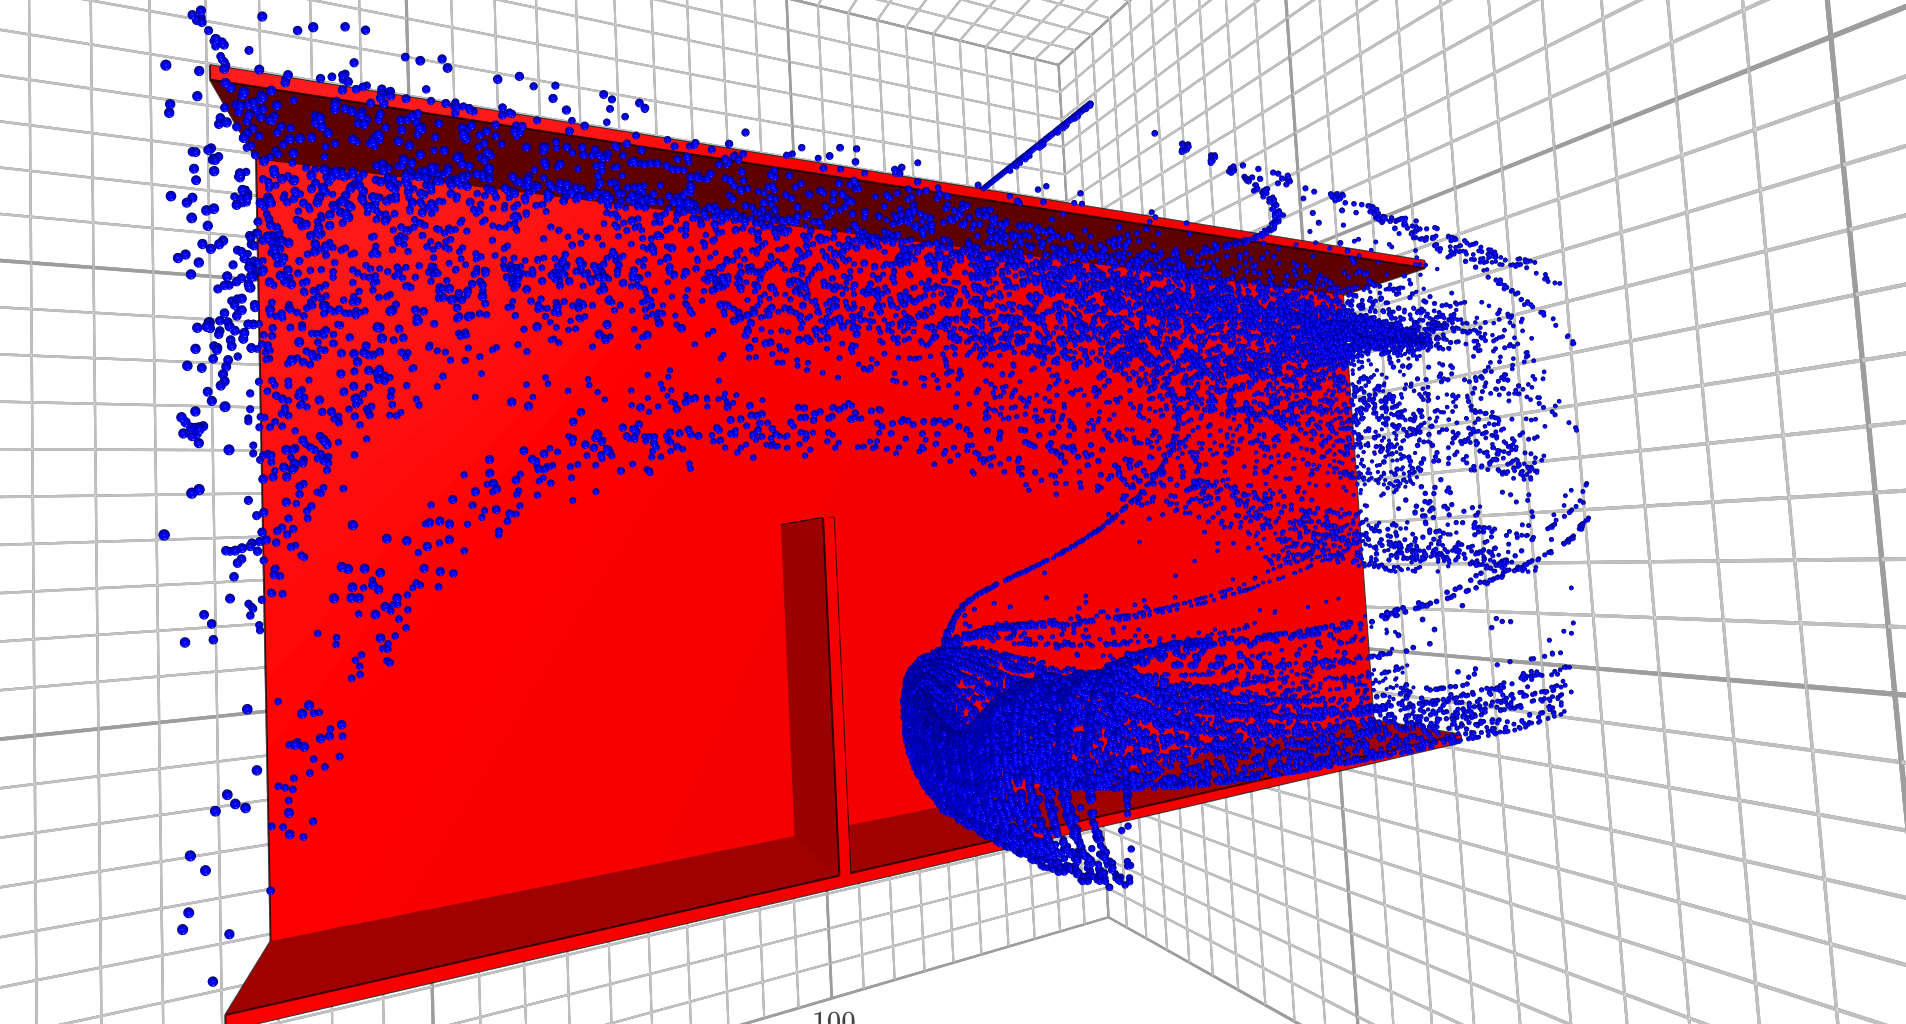
\includegraphics[width=\textwidth,trim={0 0 0 1px},clip]{k3d_cfd2.png}
  \caption{K3D visualisation of fluid
  dynamics. Boundaries are shown using a voxel object and tracers are
  dynamically updated during simulation the notebook.}
\end{figure}
 


%%%%%%%%%%%%%%%%%%%%%%%%%%%%%%%%%%%%%%%%%%%%%%%%%%%%%%%%%%%%%%%%%%%%%%%%

\section{Implementation}

The implementation of this work took the form of contributions to shared-infrastructure projects in the Jupyter ecosystem, as well as several new software packages.

\subsection{K3D-jupyter}

\href{https://github.com/K3D-tools/K3D-jupyter}{K3D-jupyter}

The package K3D-jupyter is based on threejs as a front-end 3d library
and ipywidgets (see fig. \ref{fig:pdep}) for communication.  There exists also
experimental support for ipydatawidgets. 



\subsection{pythreejs}

\href{https://github.com/jupyter-widgets/pythreejs}{pythreejs}

\subsection{unray}

\href{https://github.com/vidartf/unray}{unray}

\subsection{ipydatawidgets and ipyscales}

\href{https://github.com/vidartf/ipydatawidgets}{ipydatawidgets}

\href{https://github.com/vidartf/ipyscales}{ipyscales}



%%%%%%%%%%%%%%%%%%%%%%%%%%%%%%%%%%%%%%%%%%%%%%%%%%%%%%%%%%%%%%%%%%%%%%%%

\appendix
\section{Screenshots}\label{screenshots}

\newcommand{\screenshot}[2]{
\begin{figure}[ht]
  \includegraphics[width=\textwidth,trim={0 0 0 1px},clip]{#1}
  \caption{#2}
\end{figure}}


\screenshot{k3d_3.png}{K3D visualisation in Jupyter. The K3D widget is
  mixed with a slider to make interactive animation of Sine-Gordon
  equation in 3d space.}
% \screenshot{pythreejs.png}{PyThreeJS scene in Jupyter}
% \screenshot{unray}{Visualizing a mesh in Jupyter with unray}
% \screenshot{scivijs}{Example of a visualisation with scivijs}
% \screenshot{ipyvolume-discretizedfield}{Micromagnetics visualisation from \taskref{with ipyvolume}

\clearpage
\section{Landscape Report}\label{landscape}
This is a survey of the landscape of 3D visualization in Jupyter Notebooks
performed in March 2017 by Vidar Tonaas Fauske,
to guide \ODK contributions to 3D visualization tools.

\subsection{Summary}

Several packages currently exist that can generate 3D visualizations in
Jupyter Notebooks. This review is intended to give a quick overview of
the current landscape (March 2017), and consider where the contributions
of OpenDreamKit (ODK) can best be directed in order to help improve the
user experience in terms of both features and ease-of-use. The packages
and technologies that will be considered are:

\begin{itemize}
\tightlist
\item
  \href{http://docs.enthought.com/mayavi/mayavi/tips.html\#using-mayavi-in-jupyter-notebooks}{mayavi}
\item
  \href{https://github.com/maartenbreddels/ipyvolume}{ipyvolume}
\item
  \href{http://vispy.org}{vispy}
\item
  \href{https://www.logilab.org/blogentry/8541176}{scivijs}
\item
  \href{https://github.com/K3D-tools/K3D-jupyter}{k3d}
\item
  \href{http://vpython.org}{vpython}
\item
  \href{http://nbviewer.jupyter.org/github/sagemanifolds/SageManifolds/blob/master/Worksheets/v1.0/SM_sphere_S2.ipynb}{Sage
  plot3d}
\end{itemize}

Below you can see a (limited) dependency graph between the different
project and technologies. The red text signifies how a kernel package
sends/communicates 3D data to the browser side.

\begin{figure}
\centering
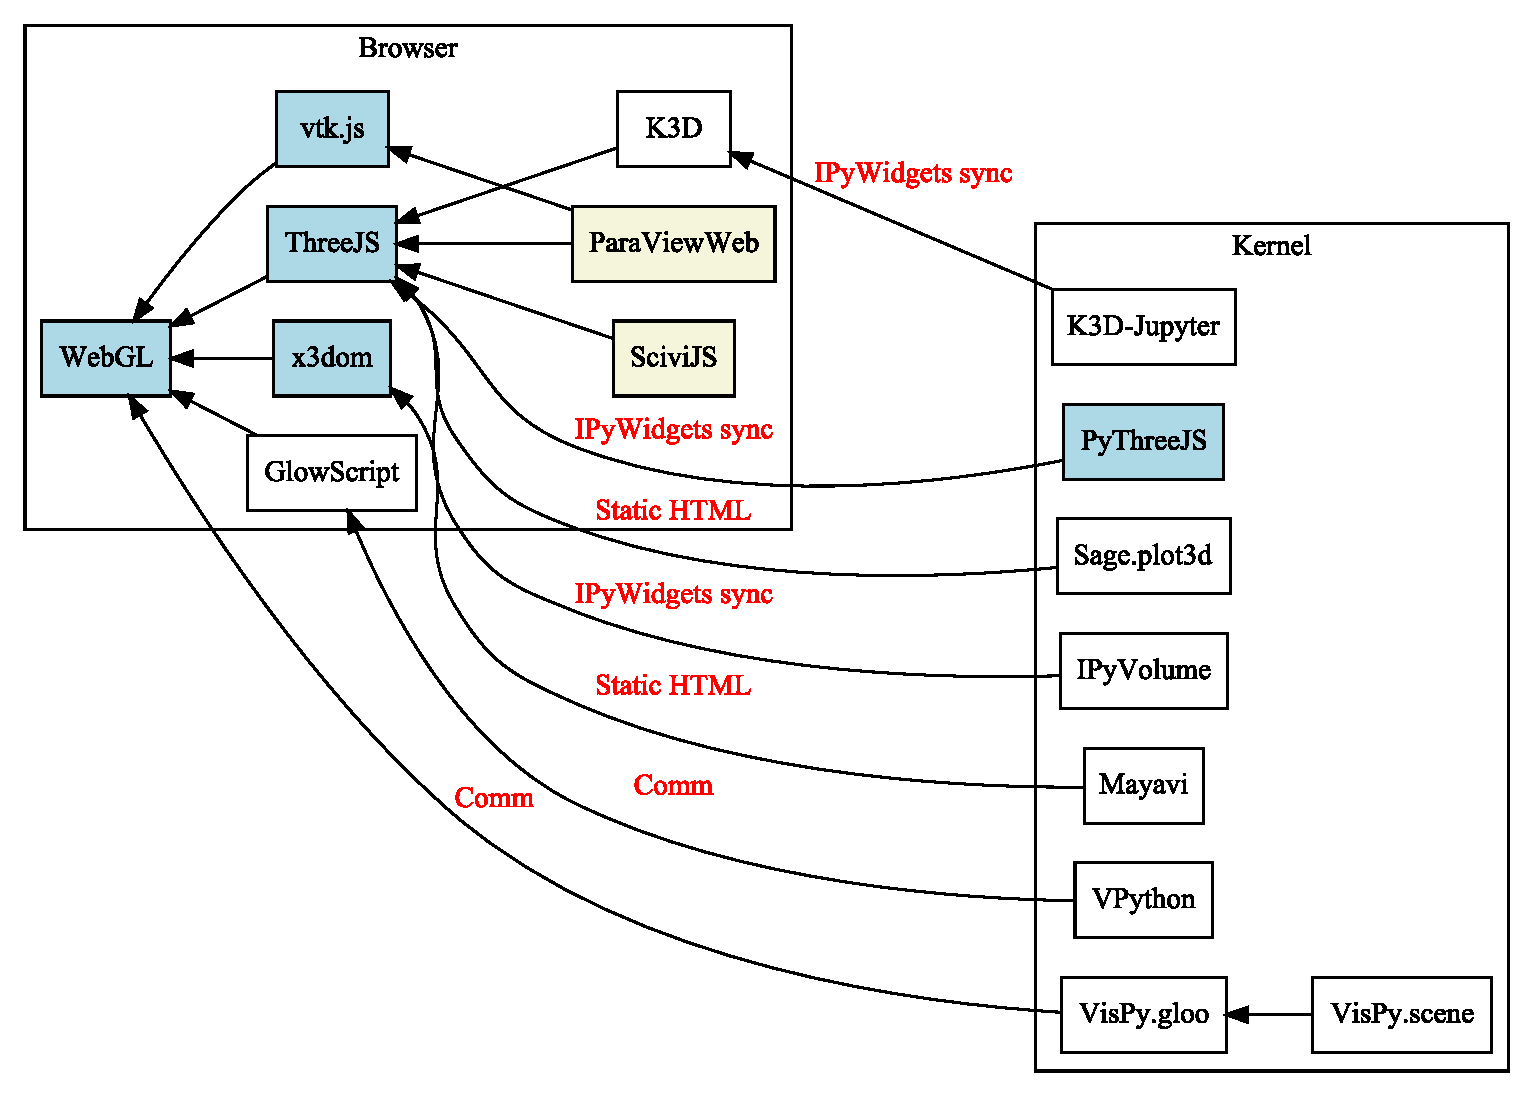
\includegraphics[width=0.6\paperwidth]{existing_tools/dependencies.pdf}
\caption{Package dependency graph}
\end{figure}

As can be seen, there is a variation in how the different projects
couples to WebGL.

    \hypertarget{observations}{%
\subsubsection{Observations}\label{observations}}

Among the packages certain patterns are repeating: - Mayavi and Sage's
plot3d both generate a blob of HTML with x3dom/ThreeJS definitions of
the model + interaction code. This is added as an output of the cell,
and it makes the visualization persistable (i.e.~the view will work the
same with or without a kernel), but it also limits interactivity. -
VPython and VisPy both use temporary displays that are controlled over
Comm. They currently require a roundtrip to the kernel for every frame
draw and/or user interaction. IPyVolume and K3D also uses a temporary
display, but avoids kernel roundtrips by using pre-defined ThreeJS view
controllers. All four packages should be able to persist the views,
e.g.~by recording the executed DOM + Javascript to the output. - Many of
the packages only supply basic inspection tools (a simple camera to
rotate/move). More advanced interactive inspection tools (varying
opacity of different parts, adding and adjusting clipping planes,
tresholding, etc.) are more rare, but could add many benefits to the
user. A possibility here would for ODK to help produce reusable
inspection tools for other visualization tools to use.

In terms of persistence, there are a few things to take into account: -
If the notebook is not trusted, JavaScript is not available, so a static
image should preferrably be saved with the notebook. - Persisting as
HTML with JavaScript is maybe the easiest as it will work out of the box
without any extensions. - Persisting e.g.~x3dom as a separate MIME-type
could enable 3D to work while untrusted (any avenues for code injection
would of course need sanitizing). Would require adding a rendrer through
an nbextension or on the Jupyter level. Adding both this MIME type and
the HTML one on a single output would be nice, but it would nearly
double the output size, which can be significant for larger
geometries/textures.

    \hypertarget{enabling-technology}{%
\subsection{Enabling technology}\label{enabling-technology}}

    \hypertarget{browser-side}{%
\subsubsection{Browser side}\label{browser-side}}

    \hypertarget{webgl}{%
\paragraph{WebGL}\label{webgl}}

The base layer in terms of enabling technology. All other packages
discussed in this report rely on this.

    \hypertarget{threejs}{%
\paragraph{ThreeJS}\label{threejs}}

A Javascript framework built on top of WebGL. ThreeJS is the most
prominent WebGL framework today.

Combining custom WebGL code with ThreeJS is not straight forward, but
adding custom shaders is reasonably easy, and ThreeJS should be a
sufficient base for most scientific visualization needs.

    \hypertarget{x3dom}{%
\paragraph{x3dom}\label{x3dom}}

A Javascript/XML framework built on top of WebGL. It takes XML as
source, and translates this into a 3D scene. While it sports a
reasonably full feature set, it has not received the same amount of
developer hours as ThreeJS, which can sometimes show. An example of a
simple feature that is missing is an orbit view controller (a ``camera''
orbiting a point, where the up axis is fixed).

    \hypertarget{vtk.js}{%
\paragraph{vtk.js}\label{vtk.js}}

Aims to be (a subset of) VTK built on WebGL. Official project by
Kitware, which plan to transition ParaViewWeb from ThreeJS to it over
time.

    \hypertarget{kernel-side-python}{%
\subsubsection{Kernel side (Python)}\label{kernel-side-python}}

    \hypertarget{pythreejs}{%
\paragraph{PyThreeJS}\label{pythreejs}}

A Python bridge to ThreeJS by syncing IPyWidgets.

\begin{quote}
\emph{``This is meant to be a low-level wrapper around three.js. We hope
that others will use this foundation to build higher-level interfaces to
build 3d plots.''}
\end{quote}

    \hypertarget{higher-level-interfaces}{%
\subsection{Higher level interfaces}\label{higher-level-interfaces}}

    \hypertarget{mayavi}{%
\subsubsection{Mayavi}\label{mayavi}}

Mayavi is a high-level interface on top of VTK. It uses x3dom to handle
3D in browser, but also supports a \texttt{png} backend.

Mayavi produces a static HTML output with an x3dom scene generated by
VTK's X3DExporter. VTK also has a WebGLExporter, which is currently not
used by Mayavi.

\hypertarget{installation}{%
\paragraph{Installation}\label{installation}}

Depends on VTK (\textgreater{}= 5.0) with Python wrappers installed. Not
straight forward to get on all Windows distrubutions, but works nicely
with conda.

The docs says to enable x3dom by installing Mayavi as a notebook
extension, but this has errors. It also bundles an outdated version of
x3dom (bugs out on high-DPI monitor). Simply not installing the Mayavi
nbextension will load the x3dom javascript dynamically from x3dom.org,
which works fine.

\hypertarget{strengths-and-weaknesses}{%
\paragraph{Strengths and
weaknesses}\label{strengths-and-weaknesses}}

Strengths: - Mature package for generating 3D visualization. - Relies on
exporting capabilities of underlying VTK, meaning it should be
reasonably robust. - Output persisted naturally.

Weaknesses: - Requires full re-plot for any changes to the VTK scene;
limited chances for interactivity via e.g.~IPyWidgets. - Requires VTK
installation.

\hypertarget{license}{%
\paragraph{License}\label{license}}

BSD 3-clause

\hypertarget{possible-contributions}{%
\paragraph{Possible contributions}\label{possible-contributions}}

\begin{itemize}
\tightlist
\item
  Make a separate notebook/jupyterlab renderer for x3dom MIME type?
\item
  Also add a static PNG snapshot to output MIME bundle.
\end{itemize}

    \hypertarget{ipyvolume}{%
\subsubsection{IPyVolume}\label{ipyvolume}}

Higher-level package for quickly creating interactive 3D plots of volume
and scatter data. Started December 2016, so still very new.

\hypertarget{installation}{%
\paragraph{Installation}\label{installation}}

Simple pip install. Package is pure Python + npm package for notebook
extension. Dependencies like Pillow are not pure Python.

Also available on conda.

\hypertarget{strengths-and-weaknesses}{%
\paragraph{Strengths and
weaknesses}\label{strengths-and-weaknesses}}

Strengths: - Integrates well into existing Jupyter environment by
building on top of IPyWidgets. - Good interactivity. - Support for
animations (although limited) with interpolation between frames.

Weaknesses: - Limited capabilities (no lines / surface plotting, no
exploration with e.g.~clip planes, etc.). - Features still need ironing
out / polishing to mature.

\hypertarget{license}{%
\paragraph{License}\label{license}}

MIT

\hypertarget{possible-contributions}{%
\paragraph{Possible contributions}\label{possible-contributions}}

\begin{itemize}
\tightlist
\item
  Help mature existing plotting tools.
\item
  Add other high-level functionality like 3D lines / surfaces? That
  might be outside the scope of the package, but a package that does
  something like this might benefit from the communication framework.
\item
  Add interactive exploration controls (clip planes etc.) based on
  IPyWidgets.
\end{itemize}

    \hypertarget{k3d}{%
\subsubsection{K3D}\label{k3d}}

Described as a \emph{``3D visualization library''}. The specifics of K3D
was not readily apparent, as its documentation is rather thin. However,
the following can be gleamed from the code/examples:

\begin{itemize}
\tightlist
\item
  K3D is intended as a Javascript library for scientific plotting
  (high-level API).
\item
  It uses ThreeJS as a backend (currently the only backend).
\item
  K3D-Jupyter is meant to shim the K3D interface to Jupyter using an
  nbextension (and implements an IPython client using IPyWidgets).
\end{itemize}

K3D might be overlapping in purpose with vtk.js.

\hypertarget{installation}{%
\paragraph{Installation}\label{installation}}

No release on PyPI/conda yet. Was able to install it from repository
after mucking around with it manually.

\hypertarget{strengths-and-weaknesses}{%
\paragraph{Strengths and
weaknesses}\label{strengths-and-weaknesses}}

Strengths: - Integrates well into existing Jupyter environment by
building on top of IPyWidgets. - Repository control is within control of
ODK participant(s), potentially avoiding conflicts of interest with
other package maintainers.

Weaknesses: - Still immature project. - Installation and documentation
needs work.

\hypertarget{license}{%
\paragraph{License}\label{license}}

MIT

\hypertarget{possible-contributions}{%
\paragraph{Possible contributions}\label{possible-contributions}}

\begin{itemize}
\tightlist
\item
  Bring installation/distribution in line with ``Jupyter standard''.
\item
  Ensure optimal use of Jupyter protocol for data transfer across
  kernel/browser interface.
\item
  Documentation.
\item
  Help mature package.
\end{itemize}

    \hypertarget{vispy}{%
\subsubsection{VisPy}\label{vispy}}

VisPy.app / VisPy.gloo: gloo is a python -\textgreater{} GL abstraction
layer, that supports talking to a WebGL context.

VisPy.scene: High-level visualization interface built on top of gloo.
Still in development, possibly abandoned.

\hypertarget{installation}{%
\paragraph{Installation}\label{installation}}

\hypertarget{strengths-and-weaknesses}{%
\paragraph{Strengths and
weaknesses}\label{strengths-and-weaknesses}}

Strengths: - Somewhat low-level GL/WebGL access from Python via GLIR
(low-level abstraction on top of various versions of GL/shader
language). - Same interface whether you want to use local GL (in e.g.~a
Qt window) or WebGL in Notebook.

Weaknesses: - Yet another interface wrapper for GL. - User interaction
and timer loops always has to round-trip to kernel side from browser. -
Development seems to has stagnated:

\begin{figure}
\centering
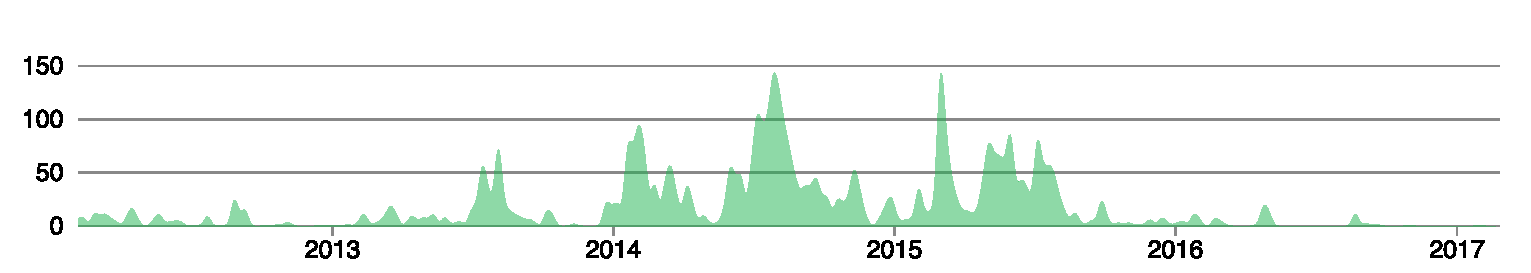
\includegraphics[width=0.6\paperwidth]{existing_tools/vispy_activity.pdf}
\caption{VisPy activity graph}
\end{figure}

\hypertarget{license}{%
\paragraph{License}\label{license}}

BSD 3-Clause

\hypertarget{possible-contributions}{%
\paragraph{Possible contributions}\label{possible-contributions}}

\begin{itemize}
\tightlist
\item
  Take over development of high-level part.
\item
  Add view controllers and inspectors to avoid round-trips to kernel
  when in browser.
\item
  Make persisting outputs.
\end{itemize}

    \hypertarget{scivijs}{%
\subsubsection{SciviJS}\label{scivijs}}

A node based framework for inspecting/deforming/shading ThreeJS based
geometry. Might overlap in purpose with
\href{https://kitware.github.io/paraviewweb/}{ParaViewWeb}.

\hypertarget{installation}{%
\paragraph{Installation}\label{installation}}

Installation via \texttt{npm}: unproblematic.

\hypertarget{strengths-and-weaknesses}{%
\paragraph{Strengths and
weaknesses}\label{strengths-and-weaknesses}}

Strengths: - Inspection/exploration tools. - Based on ThreeJS.

Weaknesses: - Still undocumented.

\hypertarget{license}{%
\paragraph{License}\label{license}}

\href{https://opensource.org/licenses/ISC}{ISC}

\hypertarget{possible-contributions}{%
\paragraph{Possible contributions}\label{possible-contributions}}

\begin{itemize}
\tightlist
\item
  Enable SciViJS as an inspector for other packages using (Py)ThreeJS
\item
  Help mature the code and add features as needed.
\end{itemize}

    \hypertarget{vpython}{%
\subsubsection{VPython}\label{vpython}}

Uses GlowScript (sister project) on the browser side to render GL, and
VPython on the kernel side to generate scenes. Implements most things
itself, which means everything is tailored for its purpose, but it loses
out on the benefits of larger libraries. Code can be a bit hard to
follow.

\hypertarget{installation}{%
\paragraph{Installation}\label{installation}}

Easy install (pip install vpython worked well). A little hard to figure
out which repository/package is the latest. I think this repository is
the main one: https://github.com/BruceSherwood/vpython-jupyter, and
\texttt{vpython} the PyPI package to install. Glowscript is bundled in a
minified version in VPython repository.

\hypertarget{strengths-and-weaknesses}{%
\paragraph{Strengths and
weaknesses}\label{strengths-and-weaknesses}}

Strengths: - Few dependencies. - Active development.

Weaknesses: - Uses quite a lot of browser CPU when idle. - Difficult to
understand code base for someone new.

\hypertarget{license}{%
\paragraph{License}\label{license}}

MIT

\hypertarget{possible-contributions}{%
\paragraph{Possible contributions}\label{possible-contributions}}

\begin{itemize}
\tightlist
\item
  Clean up documentation / repositories as someone coming from outside
  with fresh eyes.
\item
  Refactor codebase to ease outside contributions?
\item
  Make persisting outputs
\end{itemize}

    \hypertarget{sage.plot3d}{%
\subsubsection{Sage.plot3d}\label{sage.plot3d}}

Uses its own code to convert 3D plots to ThreeJS code, which it embeds
into a static HTML output. As such, it is similar to Mayavi, but is
based on ThreeJS instead of x3dom.

    \hypertarget{vtk.js---jupyter}{%
\subsubsection{VTK.js - Jupyter?}\label{vtk.js---jupyter}}

An option would be to implement Jupyter/IPython bindings for vtk.js.

\hypertarget{strengths-and-weaknesses}{%
\paragraph{Strengths and
weaknesses}\label{strengths-and-weaknesses}}

Strengths: - vtk.js has backing of big organization and has a mature
API. - Interface should be familiar to those experienced with VTK. -
Should make it easy to put ParaViewWeb on top for
exploration/inspection. - Possibly good integration with Mayavi?

Weaknesses: - Mostly at mercy of Kitware and their attitude towards
vtk.js (e.g.~if they decide to drop it or it is poorly supported). -
Unkown time-horizon.

    \hypertarget{concluding-remarks}{%
\subsection{Concluding remarks}\label{concluding-remarks}}

The following features would all be wanted from a 3D visualization
toolkit for use in Jupyter:

\begin{itemize}
\tightlist
\item
  It should offer a complete API for plotting 3D visualizations.
\item
  More specialized visualizations should hopefully be able to build on
  top of the API for their own purposes.
\item
  It should be open to interactive behavior, while avoiding sending
  redundant information between the kernel and browser.
\item
  It should have tools for inspection/exploration that does not require
  a round-trip to the kernel (syncing inspection parameters is ok, but
  this should not block).
\item
  It would be beneficial if the API could also be used to generate plots
  outside of the Notebook enviornment as well, or at least be able to
  switch to such a tool with little effort.
\item
  The API can benefit greatly by being similar to existing patterns
  (e.g.~Matplotlib or Mayavi/VTK), to ease the learning-curve for new
  users.
\end{itemize}

It is not necessarily aparent which package or combination of packages
are the best to achieve all of these, but the following are examples of
possible solutions: 0. IPyVolume + SciviJS. Uncertain difficulty of
SciviJS integration. 0. K3D + SciviJS 0. ``Jupyter-VTK'': Jupyter
bindings to VTK.js + ParaWebView. Might include Mayavi.


\end{document}
